% Chapter 4

\chapter{Goanna: Finding All Type Errors Using Minimal Correction Sets} \label{chap:goanna} 

Statically-typed languages have gained popularity in the mainstream programming world \cite{stack_exchange_inc_stack_nodate}. Many new languages have been designed with strict type systems, while others have introduced static typing through external tools. Numerous studies indicate that programming with strongly-typed languages can prevent certain errors \cite{bogner_type_2022}, enhance code quality \cite{mayer_empirical_2012}, and reduce maintenance costs \cite{kleinschmager_static_2012} compared to similarly positioned dynamic languages \cite{bogner_type_2022}. Despite their increasing popularity and benefits, challenges persist in the real-world adoption of these languages \cite{zeng_identifying_2019}. The steep learning curve of complex type systems remains an obstacle to their adoption. 

Haskell is renowned for its expressive and robust type system. It enables programmers to model complex problems as constructs and relations within type systems and develop robust programs in a type-driven style. Historically, many type system innovations initially introduced by Haskell \cite{hudak_history_2007}, including algebraic data types, type inference, and type classes, have now found their way into mainstream programming languages \cite{noauthor_introduction_nodate,noauthor_documentation_nodate,noauthor_defining_nodate}.
    
However, Haskell is also known for its steep learning curve and unforgiving type errors. Numerous research efforts have attempted to address these challenges \cite{tirronen_understanding_2015,chen_counter-factual_2014,heeren_helium_2003,zhang_diagnosing_nodate,zhang_sherrloc_2017,lerner_searching_2007}. The type errors generated by the most commonly used Haskell compiler, GHC (Glasgow Haskell Compiler), often lead to confusion among novice users, and sometimes experts.

    To address these challenges of diagnosing and fixing type errors in Haskell, we present a new tool: \textit{Goanna}. Goanna is a Haskell type checker based on program slicing and Minimal Correct Set (MCS) enumeration. Compared to traditional type-checking tools, Goanna provides improved type error reporting by giving a comprehensive list of possible causes and suggesting valid fixes for each cause.  Goanna differs from past type debugging systems (as reviewed in Section \ref{sec:related-work}) through its use of Minimal Correction Subsets (MCS), where a single MCS represents a complete set of locations that constitutes a possible cause.

	To further enhance Goanna's support for type-error resolution, we provide optimization strategies (Section~\ref{sub:optimization}) to identify and reduce the unhelpful suggestions, as well as ranking heuristics (Section~\ref{sub:ranking}) to reduce the steps needed to achieve a successful resolution. Additionally, we provide Goanna-IDE, an interactive debugging front-end designed to efficiently navigate and interpret Goanna's type error diagnosis.

    We conducted empirical studies that evaluated Goanna's accuracy (Section \ref{sub:eval-accuracy}), conciseness (Section \ref{sub:eval-conciseness}), and performance (Section \ref{sub:eval-performacne}). Our evaluation reveals that compared to other type-checking tools, Goanna consistently provides accurate error diagnostics and correct fixes in its top suggestions. We also demonstrate that Goanna generally offers a concise list of possible causes, thanks to its cause optimization process. While Goanna may not consistently provide instantaneous results for real-time feedback, it can deliver on-demand diagnoses when programmers require additional assistance.
    

    The key contributions of this research include:
    \begin{itemize}
        \item Goanna, a Haskell type checker with improved error reporting based on MCS enumeration and program slicing;
        \item Goanna-IDE, an interactive type error debugging interface for Haskell; 

        \item A collection of heuristics and optimization techniques to enhance MCS-based type error reporting; and

        \item An evaluation of Goanna's accuracy, conciseness, and performance.
    \end{itemize}

  The techniques we used in Goanna, such as MCS enumeration and heuristics for ranking possible causes, are not exclusive to Haskell. Rather, they are applicable to statically typed programming languages in general. We intentionally designed Goanna to use a module architecture that can be easily extended to support polyglot capability.
  
\section{Motivation Example}

For instance, in the program shown in Fig.~\ref{fig:motivation}, a type mismatch between a {\tt Char} type and an integer number type results in a perplexing type error for novice users. We have identified three challenges for making use of these error messages:


    \begin{enumerate}
        \item The error is fixated on one possible cause while other potential causes exist.
        \item Changing the suggested location does not completely rectify the error.
        \item Inadequate contextual information for programmers to understand how the judgment was made.

    \end{enumerate}


    \begin{figure}
        \centering
        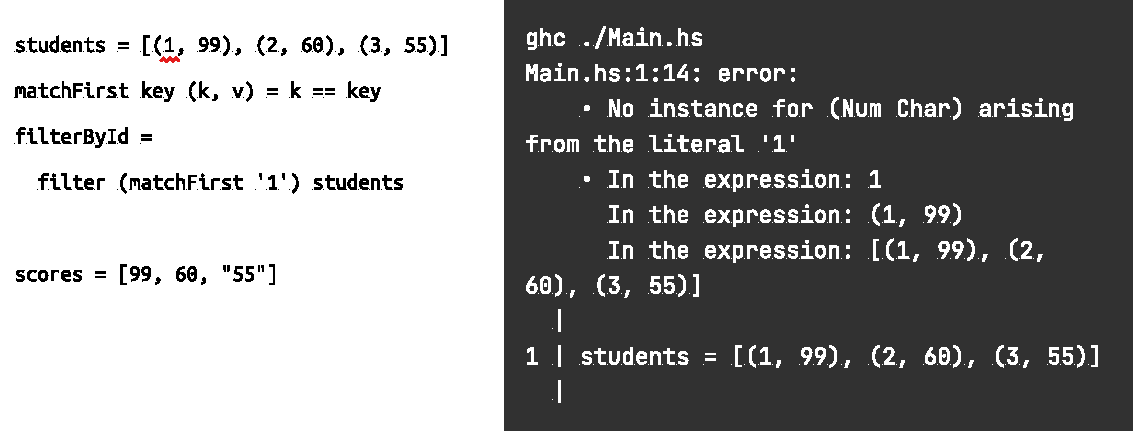
\includegraphics[width=\linewidth]{Figures/motivation}
        \caption{Inspecting a type error using the Haskell compiler GHC (Glasgow Haskell Compiler)}
        \label{fig:motivation}
    \end{figure}


\section{Feature Walkthrough}

\section{Implementation}

\section{Evaluation}

\section{Conclusion and Future Work}